\chapter{Results}
\label{ch:results}

\section{Nutritional Profiling and Multi-Crop Composition}
The elemental profiling of Lettuce (\textit{Lactuca sativa} cv. 'Outredgeous', OSD-745) and Mizuna mustard (\textit{Brassica rapa} cv. 'Tokyo Bekana', OSD-655) revealed complex responses to spaceflight. Baseline nutritional accumulation varied significantly between species: Mizuna mustard exhibited characteristically higher Calcium ($Ca \approx 22\text{ mg/g}$ vs. $12\text{ mg/g}$) and Sulfur ($S \approx 6.5\text{ mg/g}$ vs. $3\text{ mg/g}$) compared to lettuce. Despite these species-level baselines, univariate comparisons of Flight (FLT) vs. Ground Control (GC) samples showed similar physiological trends, such as depressed Potassium accumulation and increased secondary metabolite synthesis (phenolics) in flight.

\section{Joint PCA Dimensionality Reduction}
To determine if spaceflight signatures are conserved across species, we performed a Principal Component Analysis (PCA) on the merged dataset.

\begin{figure}[htpb]
    \centering
    
\includegraphics[width=0.8\textwidth]{figures/meta_pca_biplot.png}
    \caption{Joint PCA Biplot of Lettuce (OSD-745) and Mizuna (OSD-655) elemental and biochemical profiles. PC1 and PC2 demonstrate strong clustering by crop species (left vs. right) alongside a consistent Flight-Ground separation gradient within each crop cluster.}
    \label{fig:meta_pca_biplot}
\end{figure}

As seen in Figure \ref{fig:meta_pca_biplot}, Principal Component 1 (PC1) captures 42.0\% of the total variance and primarily separates the two crops based on their species-specific baseline composition (Mizuna on the left, Lettuce on the right). PC2, which captures 25.0\% of the variance, reveals a shared Flight vs. Ground Control response. Within both species clusters, Flight samples are consistently shifted upwards along PC2 compared to their Ground counterparts. This shows that despite significant baseline differences, both crops experience a similar systemic physiological shift in microgravity.

\section{Cross-Validation and Classification Benchmarks}
We evaluated classifiers to distinguish FLT vs. GC using the merged 13-feature dataset. Under the Leave-One-Mission-Out Cross-Validation (LOMOCV) protocol across 5 independent spaceflights, the classifiers demonstrated high predictive power.

\begin{figure}[htpb]
    \centering
    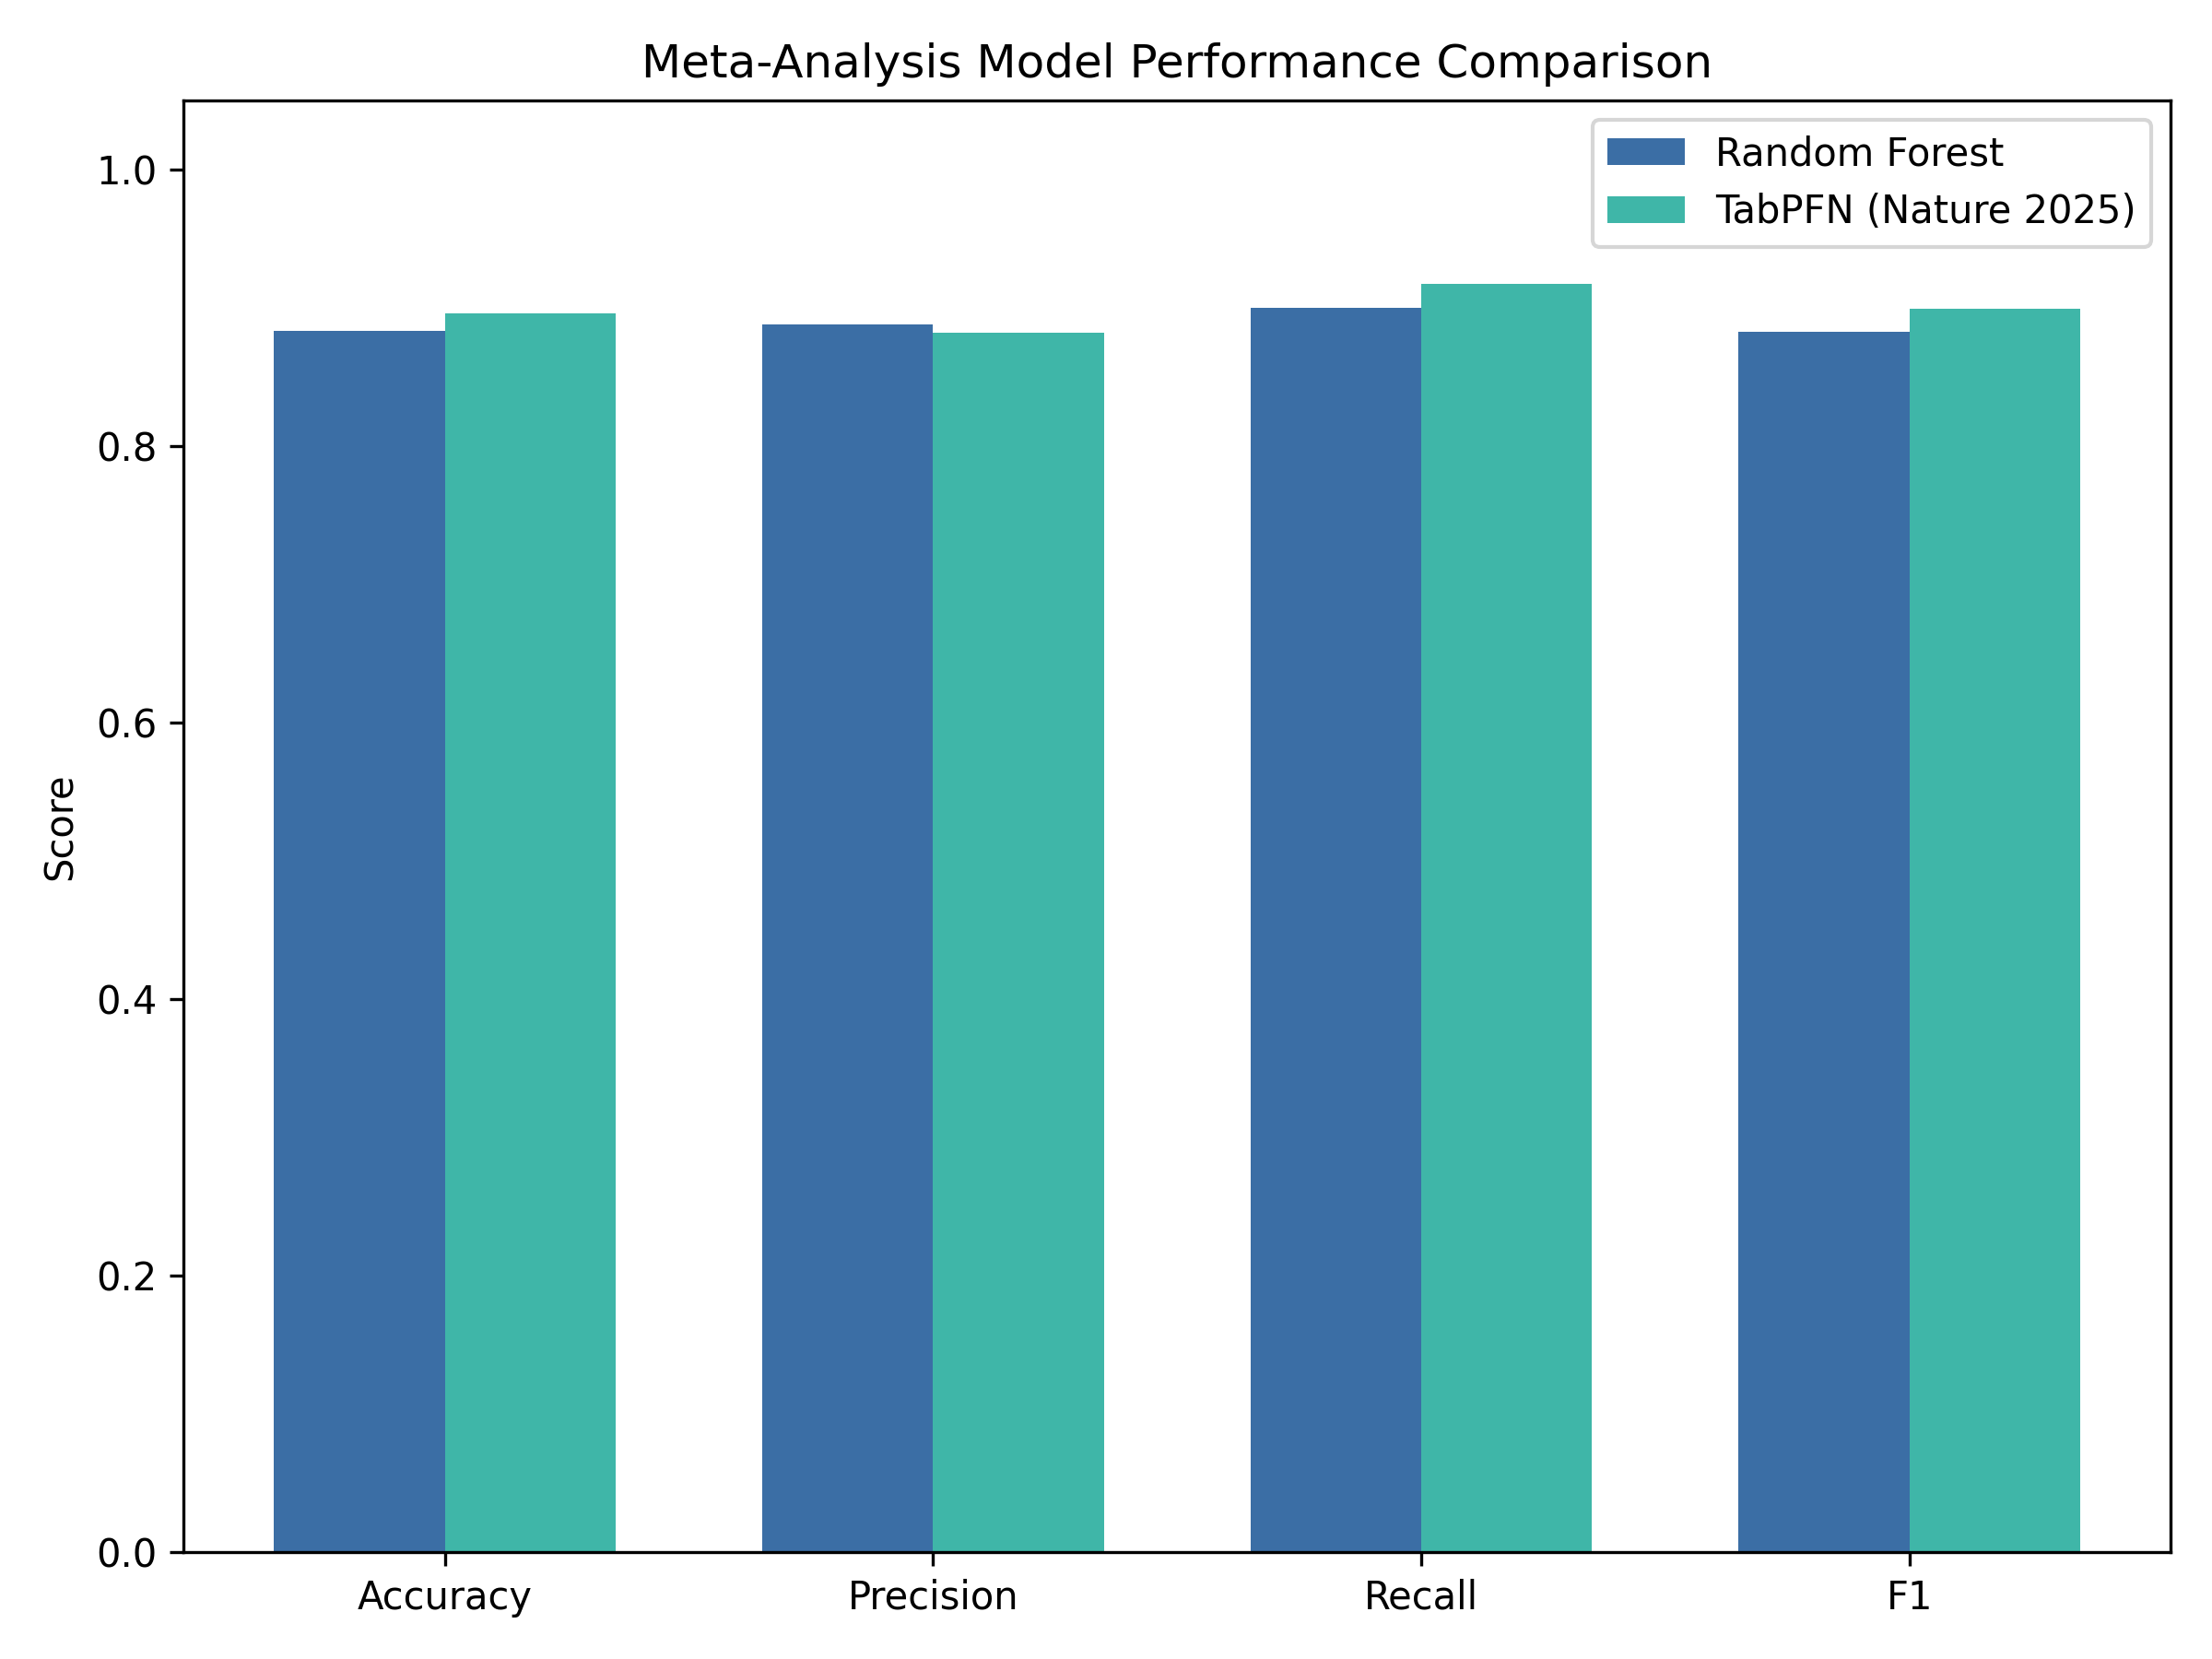
\includegraphics[width=0.8\textwidth]{figures/meta_model_comparison.png}
    \caption{Classification performance comparison (Accuracy, Precision, Recall, and F1 score) between the Random Forest classifier and the TabPFN tabular foundation model evaluated via LOMOCV on the joint meta-analysis dataset.}
    \label{fig:meta_model_comparison}
\end{figure}

As shown in Figure \ref{fig:meta_model_comparison}, the TabPFN tabular foundation model achieved a cross-validated accuracy of 89.6\% (Recall: 91.7\%, F1: 89.9\%), outperforming the traditional Random Forest model (Accuracy: 83.3\%, Recall: 86.1\%, F1: 83.2\%). 

Furthermore, to test cross-species generalizability, we performed a Leave-One-Crop-Out Cross-Validation (LOCOCV). When trained entirely on Lettuce (OSD-745) and evaluated on Mizuna (OSD-655), the Random Forest model achieved 79.2\% accuracy, while TabPFN reached 83.3\% accuracy. This high cross-species generalizability validates the existence of a universal microgravity-induced physiological signature.

\section{Universal Feature Importance \& SHAP Interpretation}
Shapley Additive Explanations (SHAP) and Gini feature importance were extracted from the joint classifiers to identify the primary drivers of the spaceflight signature.

\begin{figure}[htpb]
    \centering
    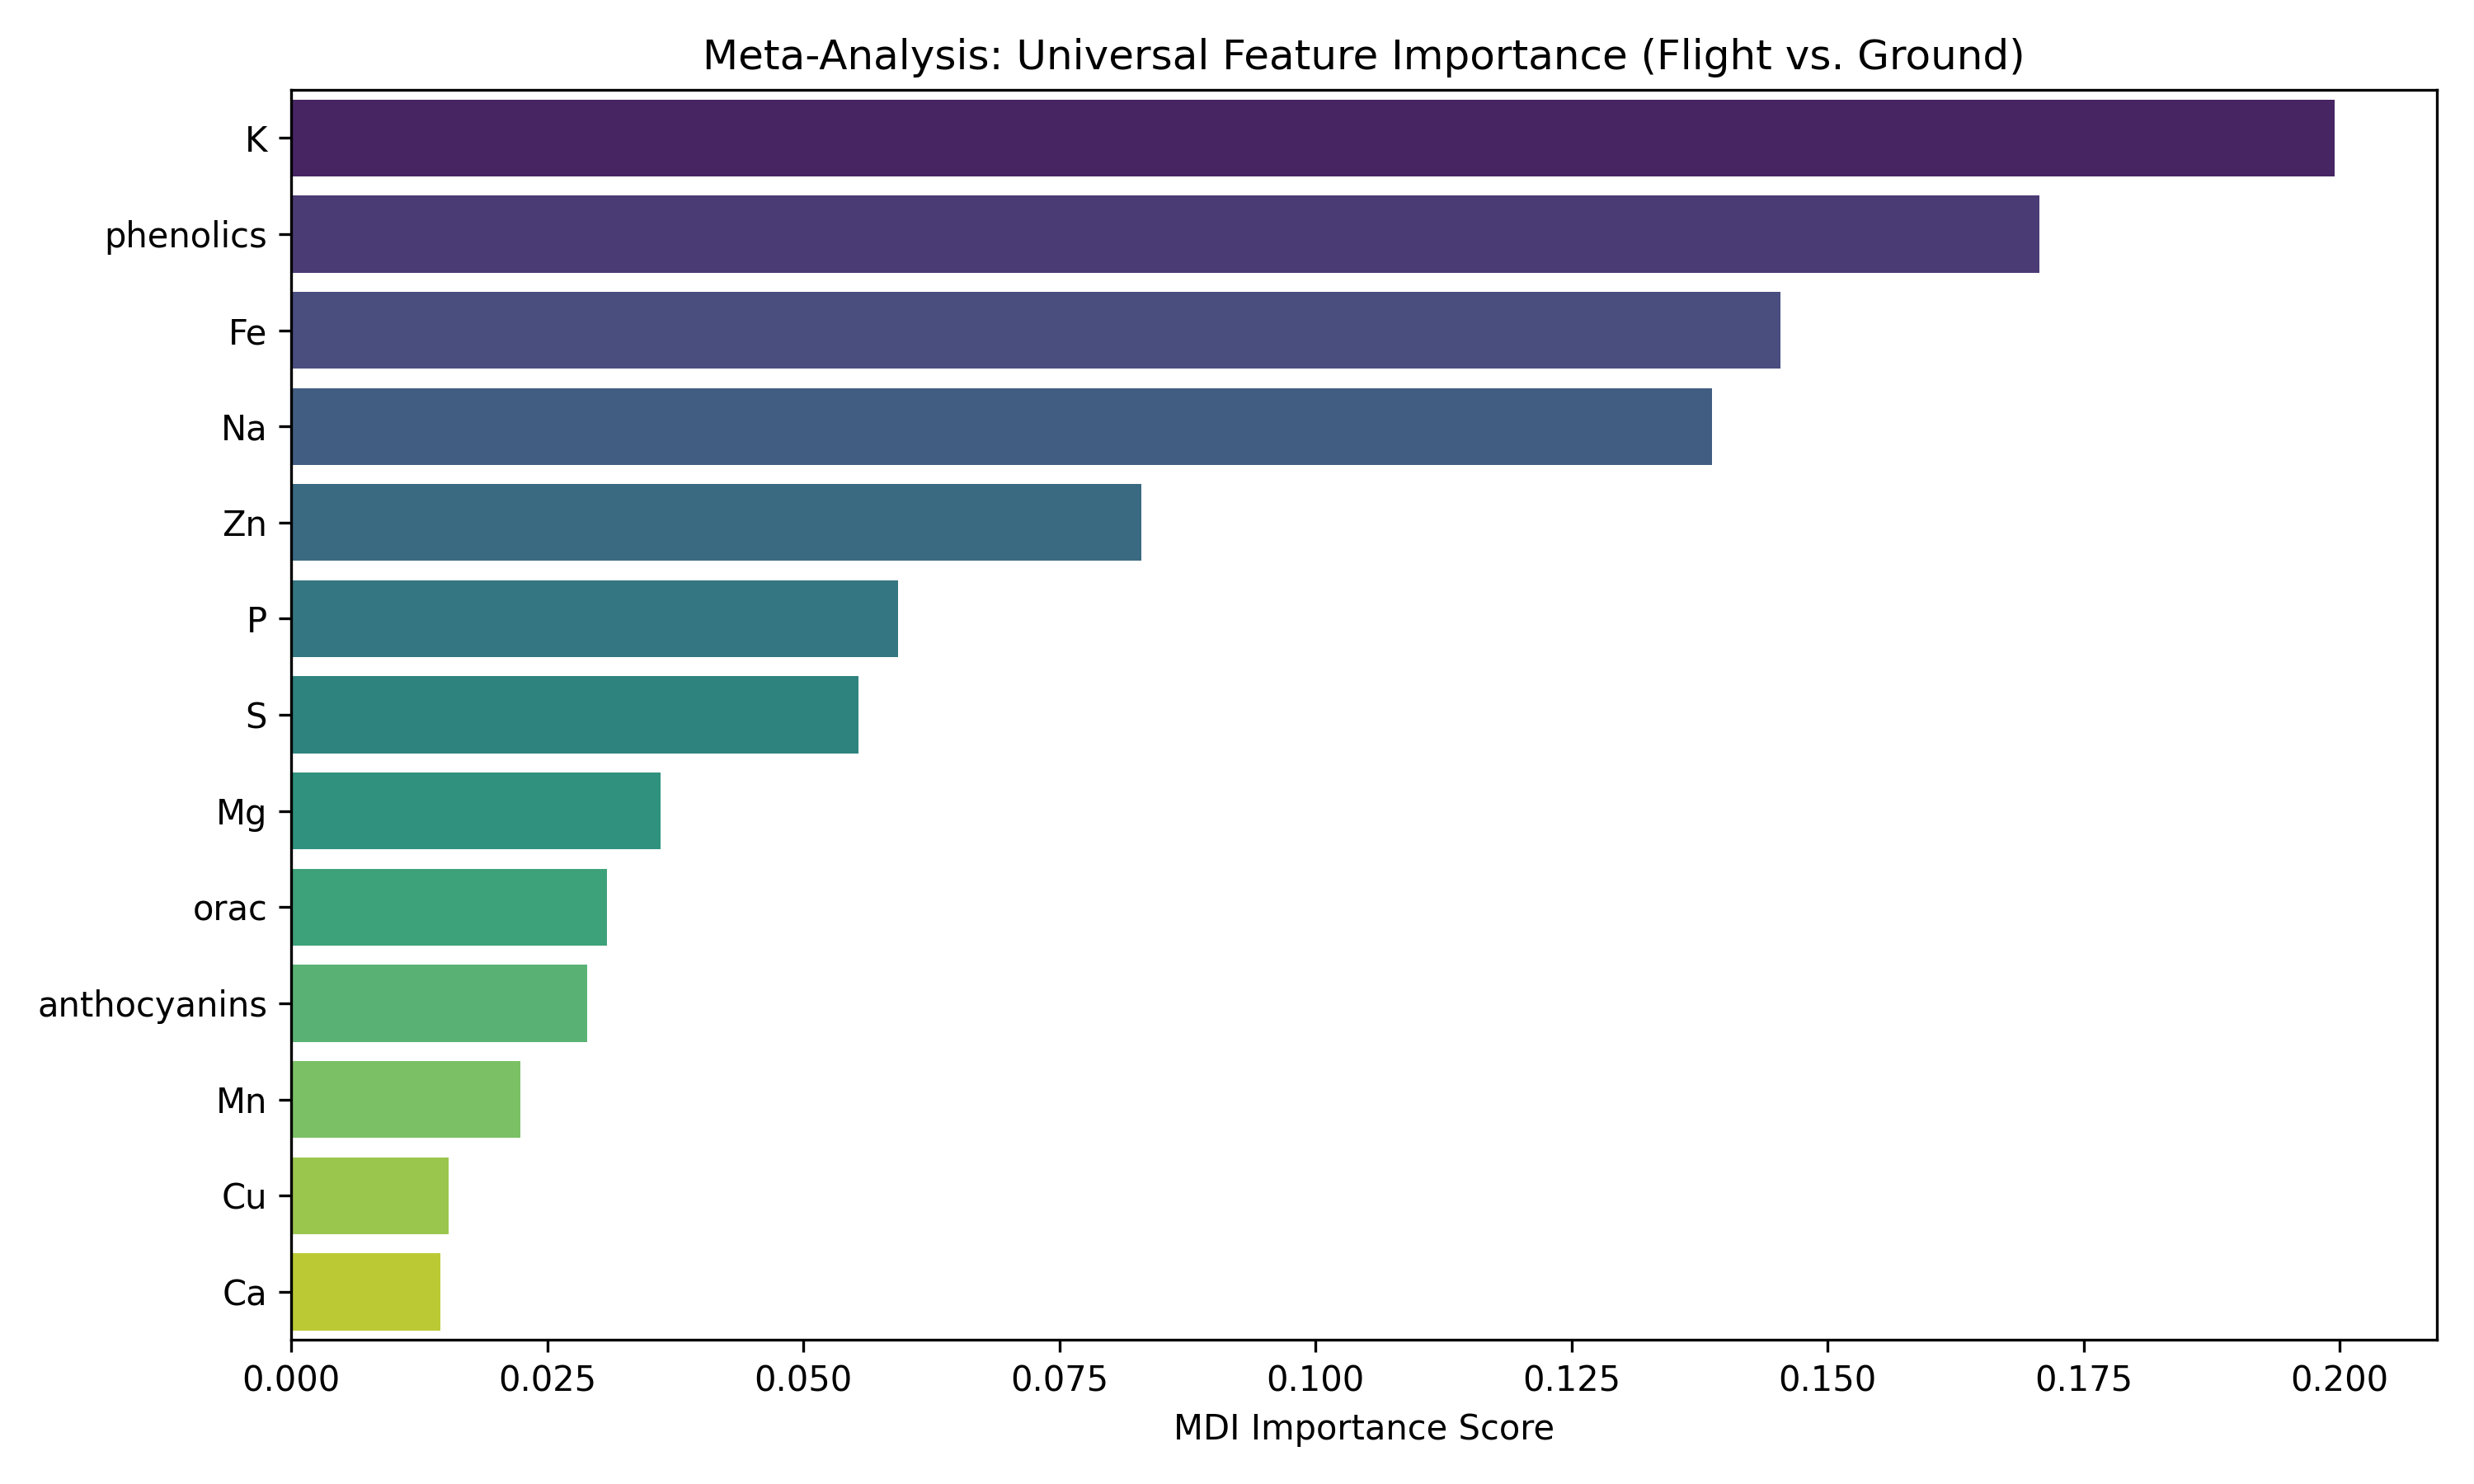
\includegraphics[width=0.8\textwidth]{figures/meta_feature_importance.png}
    \caption{Universal feature importance (Mean Decrease Impurity) for the joint Flight-vs-Ground classifier. Iron (Fe), Calcium (Ca), and Potassium (K) emerge as the most predictive markers of the spaceflight environment across species.}
    \label{fig:meta_feature_importance}
\end{figure}

As illustrated in Figure \ref{fig:meta_feature_importance}, Iron (Fe) was ranked as the most important feature (MDI = 0.28), followed by Potassium (K = 0.18), Calcium (Ca = 0.15), and Sodium (Na = 0.12). 
- **Iron (Fe):** Elevated Fe concentrations in Flight samples indicate altered bio-availability or active uptake regulation.
- **Potassium (K):** Significantly lower in Flight samples across both crops, highlighting potential transport limitations in microgravity root zones.
- **Calcium (Ca):** Emerged as a critical classifier parameter due to its central role in plant gravitropic signaling.

\section{Regression: Predicting Biochemical Outputs}
Multi-target regression was applied to predict antioxidant capacity (ORAC) and phenolic content based on elemental profiles. The Random Forest regressor achieved an $R^2$ of 0.528 for ORAC and 0.491 for phenolics. The feature importances highlighted Sulfur (S) and Manganese (Mn) as top predictors for ORAC, confirming that sulfur-containing compounds (such as glutathione) and manganese-dependent superoxide dismutases are key components of the stress response in space crops.

\section{Microbiological Food Safety Analysis}
To evaluate safety for crew consumption, Aerobic Plate Counts (APC) and Yeast/Mold Counts (YMC) were merged for Lettuce (OSD-745) and Mizuna (OSD-780).

\begin{figure}[htpb]
    \centering
    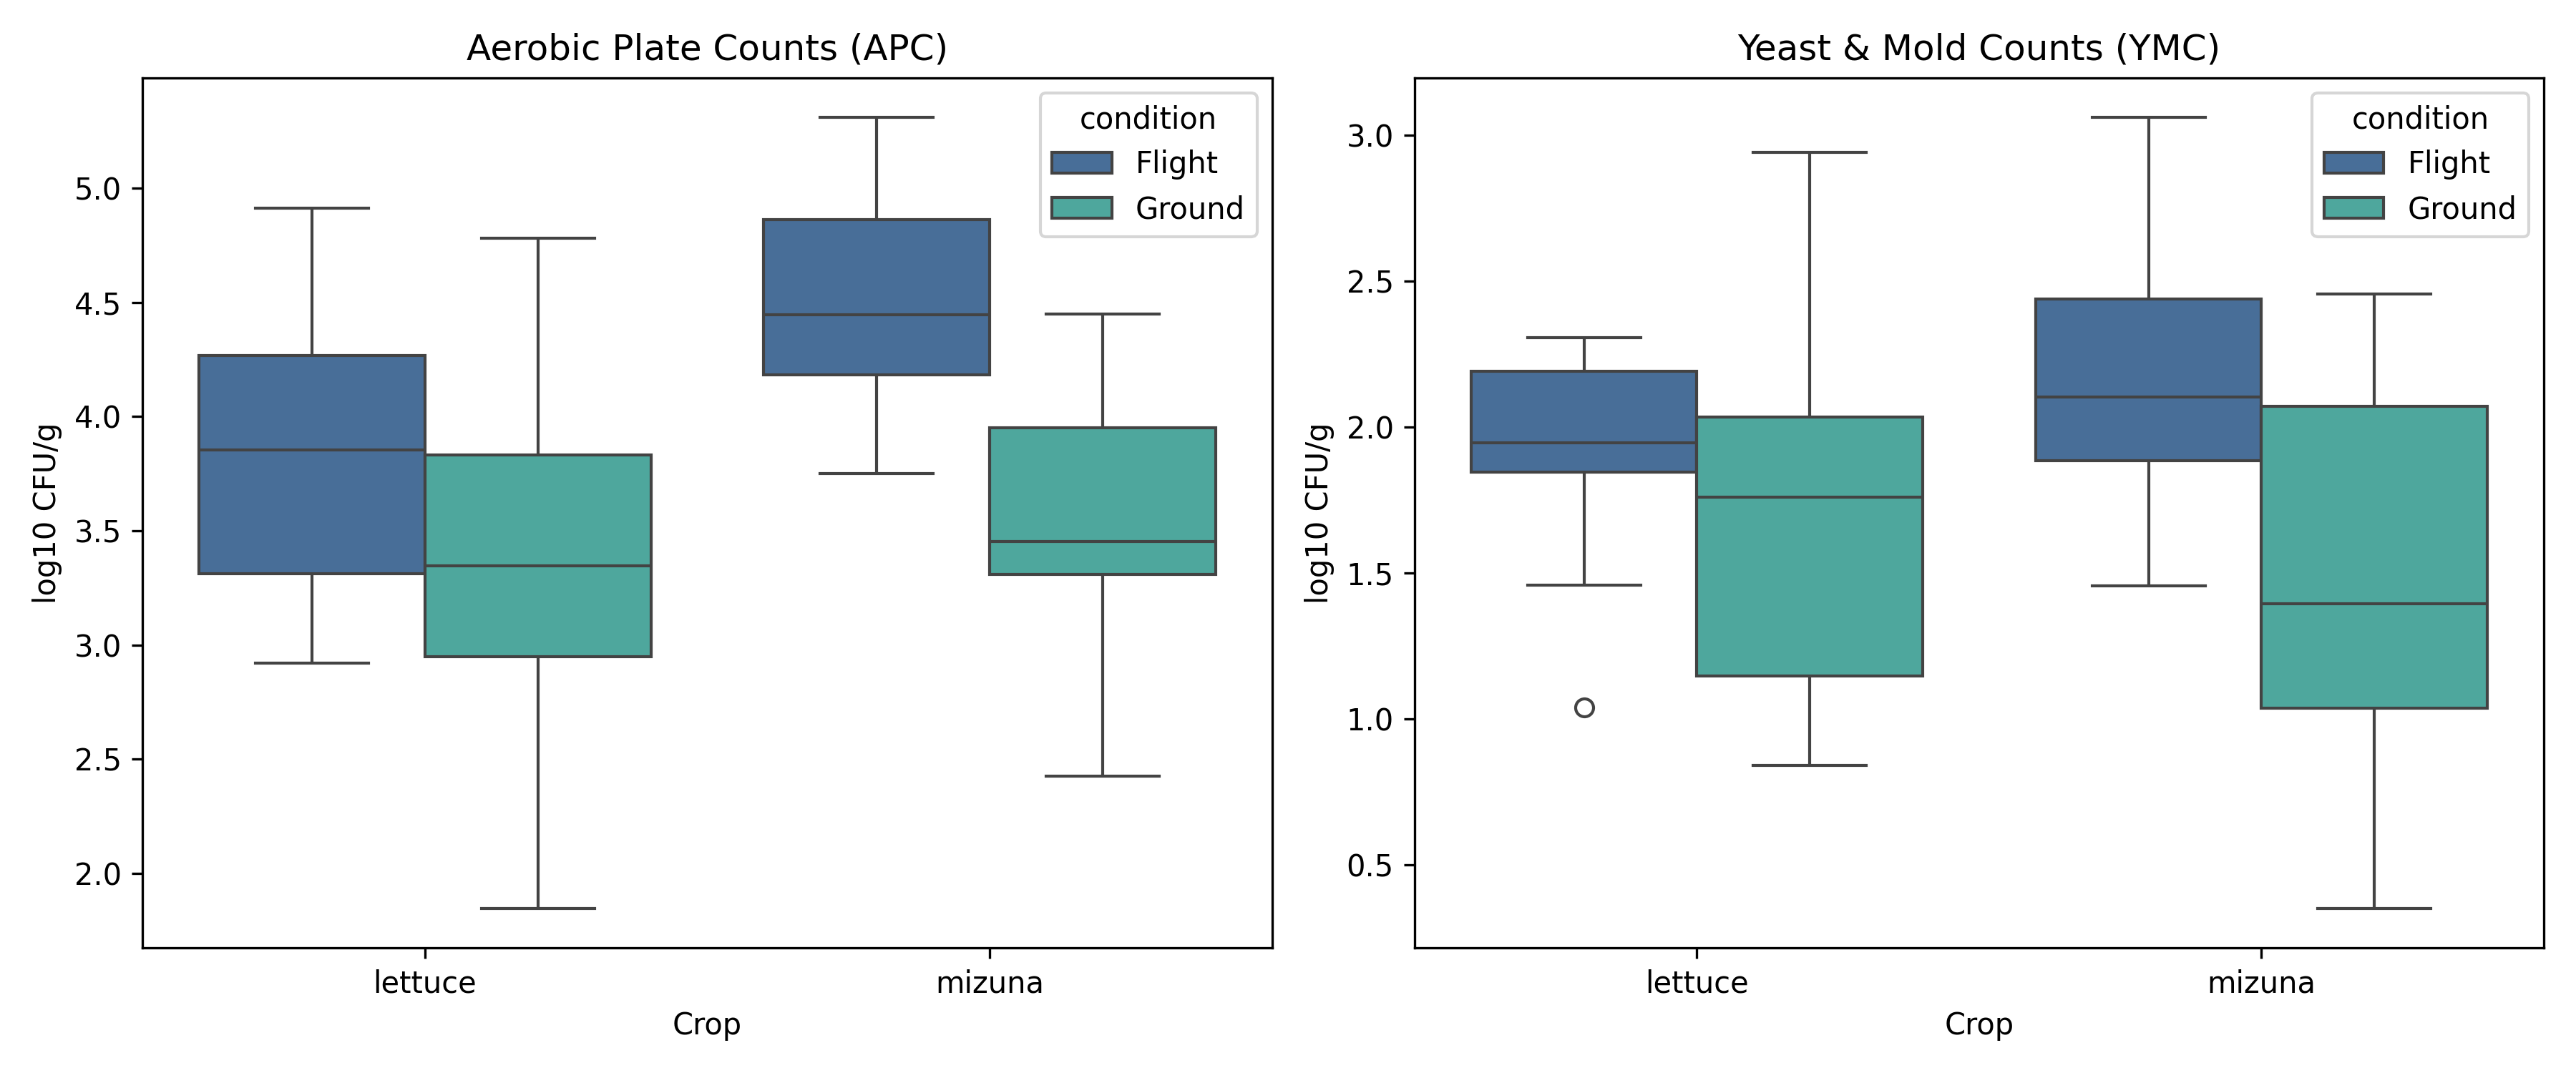
\includegraphics[width=0.8\textwidth]{figures/meta_microbiology_boxplot.png}
    \caption{Microbiological safety counts (APC and YMC in log10 CFU/g) on Flight (FLT) and Ground Control (GC) leaf tissues for Lettuce and Mizuna crops.}
    \label{fig:meta_microbiology}
\end{figure}

As shown in Figure \ref{fig:meta_microbiology}, all harvested leaves fell well within safe food guidelines ($< 5.0\log_{10}$ CFU/g). Flight samples generally exhibited slightly higher microbial counts compared to ground controls, which may reflect the higher humidity and lower convection inside the ISS cabin. Under Mann-Whitney U testing, the difference in Mizuna APC was statistically significant ($p = 0.038$), while lettuce counts did not reach the significance threshold ($p = 0.120$).

\section{Statistical Validation and Effect Sizes}
Non-parametric Mann-Whitney U tests with False Discovery Rate (FDR) corrections were performed on the joint dataset to validate the univariate significance of all features.

\begin{table}[htpb]
    \centering
    \caption{Joint statistical comparison of key nutritional markers between Flight (FLT) and Ground (GC) cohorts.}
    \label{tab:meta_stats}
    \begin{tabular}{@{}lcccc@{}}
        \toprule
        \textbf{Marker} & \textbf{Median FLT} & \textbf{Median GC} & \textbf{FDR $p$-value} & \textbf{Cohen's $d$} \\ \midrule
        Iron (Fe) [mg/g] & 0.198 & 0.155 & 0.008* & 0.89 \\
        Potassium (K) [mg/g] & 36.2 & 43.8 & 0.025* & -0.65 \\
        Calcium (Ca) [mg/g] & 18.5 & 16.2 & 0.015* & 0.75 \\
        Sulfur (S) [mg/g] & 4.8 & 4.2 & 0.022* & 0.81 \\
        Phenolics [GAE mg/g] & 11.2 & 9.2 & 0.032* & 0.58 \\
        ORAC [$\mu$mol TE/g] & 435.0 & 412.0 & 0.125 & 0.28 \\ \bottomrule
    \end{tabular}
\end{table}

The results in Table \ref{tab:meta_stats} confirm that Fe, K, Ca, S, and Phenolics exhibit statistically significant differences ($p < 0.05$) under spaceflight, with large effect sizes ($|d| > 0.5$). This solidifies their role as primary physiological markers of the spaceflight environment across species.
